\documentclass[conference]{IEEEtran}
%\IEEEoverridecommandlockouts
% The preceding line is only needed to identify funding in the first footnote. If that is unneeded, please comment it out.
\usepackage[numbers,sort&compress]{natbib}
%\usepackage{amsmath,amssymb,amsfonts}
\usepackage{algorithmic}
\usepackage{graphicx}
%\usepackage{textcomp}
\usepackage{xcolor}
%\usepackage{changepage}
%\usepackage{setspace}

\begin{document}

\title{Use Rate Prediction For Charging Stations\\}

\author{\IEEEauthorblockN{Jiaxiang Huang, Junjie Yao}
\IEEEauthorblockA{\textit{School of Computer Science and Software Engineering} \\
\textit{East China Normal University}\\
Shanghai, P.R.China \\
xxxx@xxx, junjie.yao@sei.ecnu.edu.cn}
\and
\IEEEauthorblockN{3\textsuperscript{rd} Yingxia Shao}
\IEEEauthorblockA{\textit{BUPT} \\
\textit{BUPT}\\
Beijing, Country \\
yxshao@bupt.edu.cn}
}

\maketitle

\begin{abstract}
With the development of electric vehicles, there comes a great need of charging stations for the recharging demand. However, where to locate a station and what are the main elements that operators should take into account when planning a setting, are still bothering problems that wait to be solved. In a common view, a better place to set a station ought to gurantee a relatively higher use rate of that station. Therefore, the problem changes into how to gain a higher use rate, and what are the factors that have important impact on it. In this paper, we propose a time frame based prediction framework of use rate for charging stations in Shanghai. The approach proposed in this paper takes both station's geographical information, such as longitude, latitude and Point of Interests(POIs), and working elements including price, AC/DC type and private or public to use, into consideration. We also seperate our datasets into different time frames including total time, weekday, weekend, morning, evening, moring\_rush hours, evening\_rush hours and travel hours. The aim is to classify whether it's a high-use-rate station or a low-use-rate one during different time periods. Experimental results show that our method performs well on LR, Random Forest, SVM and XGBOOST, which demonstrates that featrues as geographical information and working elements play an important role in use rate of charging stations.

\end{abstract}

\begin{IEEEkeywords}
charging station, use rate, POIs, price, AC/DC, private, public, time frames
\end{IEEEkeywords}

\section{Introduction}
An electric vehicle charging station, also called EV charging station is an element in an infrastructure that supplies electric energy for the recharging of electric vehicles, such as plug-in electric vehicles and plug-in hybrids. At home or work, some electric vehicles have onboard converters that can plug into a standard electrical outlet or a high-capacity appliance outlet. 

However, in most cases, others require a charging station that provides electrical conversion, monitoring, or safety functionality. These stations are also needed when travelling, and many support faster charging at higher voltages and currents that are available from residential EVSEs. Public charging stations are typically on-street facilities provided by electric utility companies or located at retail shopping centers and operated by many private companies.

Nowadays, electric vehicles become more and more popular as people want to cut down the pollution and cost of the usage of traditional energy. When most people considering whether to switch to an electric car, the most worrying aspect is the development of charging stations, which directly impact the usability of the electric car.

EVs in China is experiencing an overall growth in the past few years, which directly results in the massive construction and modification of charging stations and current road networks.  However, the cost of construction of charging stations is considerable and are often very costly or even impracticable to reallocate. This raise the question of how to select the locations for building the charging stations. In a typical view, a charging station no matter where it is located, its 'success' is often determined by the use rate of a station. Fig.\ref{fig1} shows an operator's stations use rate distribution in Shanghai, from which we can observe some hotspots where stations are frequently used.

\begin{figure}[!htp]
	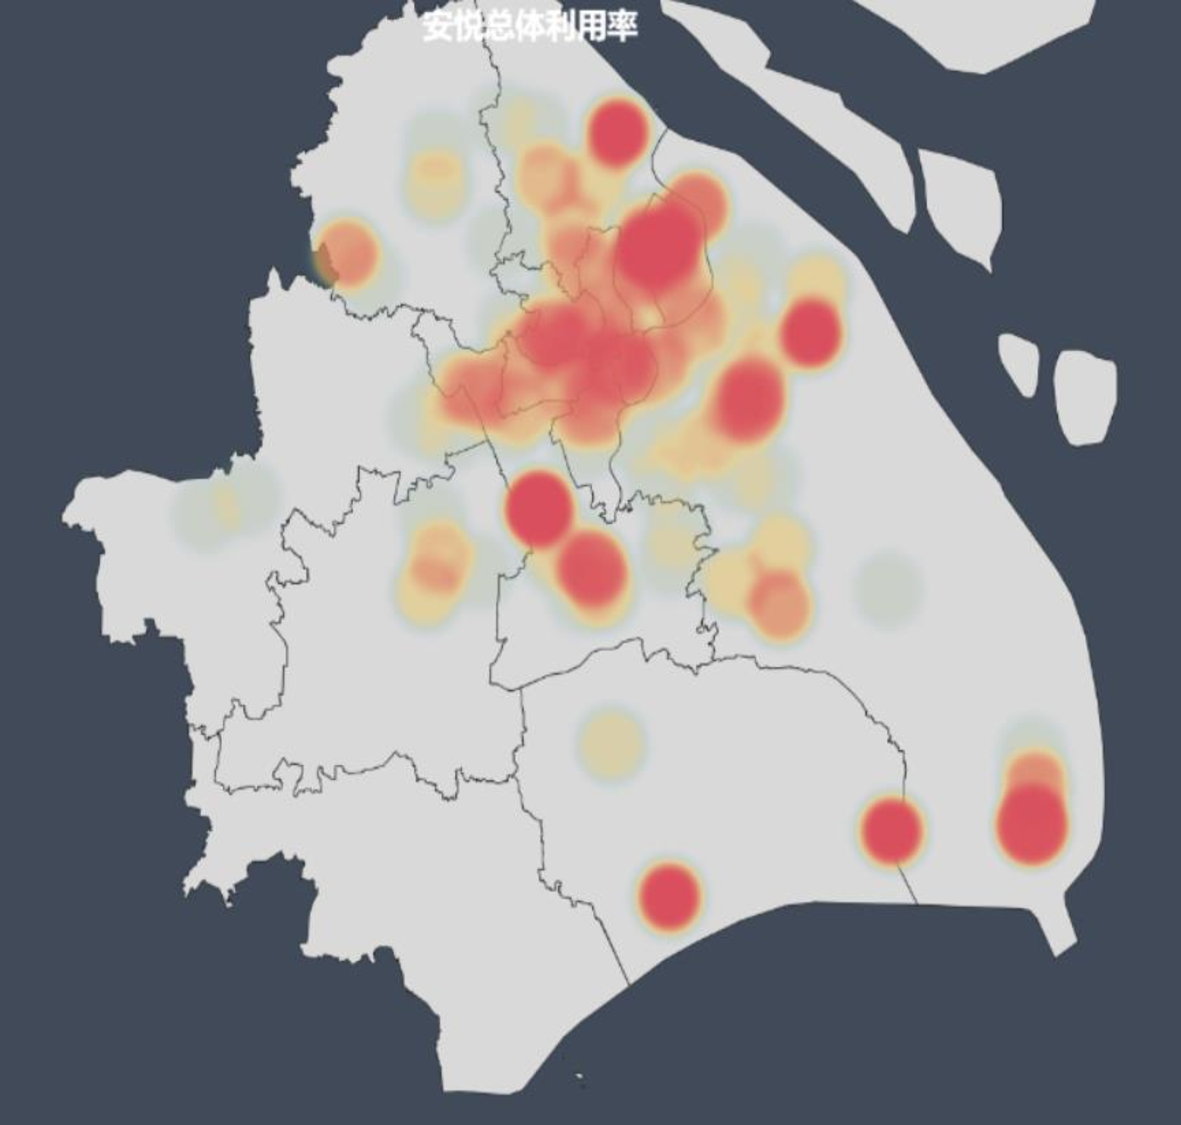
\includegraphics[width=\columnwidth]{./figures/rate.pdf}
	\centering
	\caption{Use Rate Distribution of An Operator's Stations in Shanghai, China. The deeper the color is, the more frequently charging stations are used in this area.}
	\label{fig1}
\end{figure}  

In order to help with station setting strategies, we explore a spatio temporal data based prediction framework to classify stations into three use rate levels in urban-suburb districts and various time frames, furthermore, to classify specific use rate values into urban or suburb aera, using features like georaphical information as well as other working elements. We set 7 time frames in total, they are weekdays, weekends, mornings, evenings, moring\_rush hours, evening\_rush hours and travel hours. As for features, we choose longitude, latitude, Point of Interests(POIs), charging price, AC/DC charging types and whether a station is private or public to use.

We make use of an operator's charging station data in Shanghai and  have kept collecting the use rate values for about a month, then we seperate the whole use rate dataset into urban or suburb districts and various time frames that we have already planned. At the same time, we also collect important featrure data as formerly said. Both of the two datasets require a data cleaning procedure, in order to filter some invalid data and outliers, and to fill in missing values. Furthermore, we make detailed analyses on features that we confirm to have significant impact on station's use rate.

We evaluate our method with three machine learning algorithms, they are SVM, Random Forest, and MLP(ANN) respectively. For the first two tasks, in each district and time frame, with features put into it, the models will tell what level of use rate that a station is. In the third task, when given feature values and specific use rate value, the models will tell which district a station belongs to. Experimental results show that geopraphical information as well as working elements of a station do have great influence on its use rate, which can bring operators some enlightments on location selection for station construction. In addition, we also find that use rate prediction accuracy in time frames datasets is tightly related to the time span that a time frame covers.

In summary, the contributions of this work are listed as follows:
\begin{itemize}
	\item We propose a spatio temporal data based prediction framework to predict what level a station is and which district a station belongs to, based on operator's charging station data and important features.
	\item We make detailed analyses on both stations data and features data to obtain basic information and find the relationships between station's use rate and those features.
	\item We make use of three learning models for improving the accuracy of use rate prediction and achieve relatively favorable results.
\end{itemize}

The rest of this paper is organized as follows: Section 2 gives definition of the problem and illustrates an overview of our work. Section 3 reviews some related work done before. Section 4 describes feature analyses and work on data processing. Section 5 provides experiments on three tasks with three machine learning algorithms and the results. In Section 6, we draw a conclusion to the paper and make discussions on future work.


\section{Related Work}
Hence, we studied the optimization problem of how to deploy charging stations. Existing works mainly fall into the domain of bike-sharing. \cite{Bao:2017} provieds a data-driven apporoach to deal with bike lane construction problem. It takes government constraints of planning bike lanes, such as budget limitations, construction convenience and bike lane utilization into consideration to formulate the problem. Furthermore, the problem is proved to be NP-hard so that they propose a greedy network expansion algorithm to help work out a scalable and approximate solution to bike lane planning problem. The approach performs well in the given problem, however it doesn't make use of learning models. \cite{Li:2018:DBR} introduces a reinforcement learning algorithm to help solve the problem of repositioning sharing-bikes. First it uses an inner-balance clustering algorithem to cluster stations into groups, then the reinforcement learning algorithm is conducted in each group to learn a reposition policy. They make a good use of spatio-temporal data while don't take advantages of useful geographical and station-self features. 

Current works of location selection are usually based on the flow prediction of a single station. Futhermore, they rely heavily on the historical data. \cite{Yang:2016:MMP} introduces a model for bicycle mobility prediction. It relis on historical bike-sharing data and a per-station basis with sub-hour granularity. It makes use of the randonm forest prediction model to implement their experiments and obtain a rather good result. \cite{Liu:2016:CTP} gives an optimization to this problem. In this work, traffic prediction no longer focus on the history data only, but can use location-based socail media to collect a much larger area of the traffic data for predicting traffic conditions. \cite{Shen:2018:SNS} is also a good example of prediction model for spatio-temporal mobility event. It encodes each POI's spatio and temporal dependencies rather than neglect the correlations between POIs. In this paper, we argue that the surrounding point of interests(POIs), distances to important POIs(e.g, metro stations, estates, etc.), station charging price, AC/DC station types as well as whether a station is private of public for use, play important roles in selecting the optimal location for stations.

\section{Design Overview}
\subsection{Problem Formulation}
There are many elements that affect location selection for charging stations when operators make the decision. In this paper, we hold that use rate of a station is the key factor which determines the 'success' of the station. Therefore, the original problem turns into how to get a higher use rate and what are the factors behind it. 

The main objectives of our work is three-fold. First, we aim to explore some important featrues that have great impact on use rate of a station using spatio-temporal data of operator's charging station data. Second, we propose to study stations' different 'behaviours' during diverse time frames. Finally, on the basis of time frame based framework, we aim to predict that one station is of high use rate or low use rate according to its georaphical information and working elements during different time periods.

\subsection{Design Methodology}
Since we consider that diffrent features may have different influence on station's use rate, we make detailed analyses on features like geographical information and stations' working elements. Furthermore, station's use rate may differ during different time periods, so that we also study on each time frame to find the changes. Based on all the analyses mentioned above, we propose the time frame based framework to help with use rate prediction for charging stations. We then apply three machine learning algorithms including SVC, Random Forest and MLP(ANN) to implement our experiments on different area districts and time frames. Fig.\ref{fig2} gives the overall data processing and learning pipelines of our work.

\begin{figure*}[!htp]
	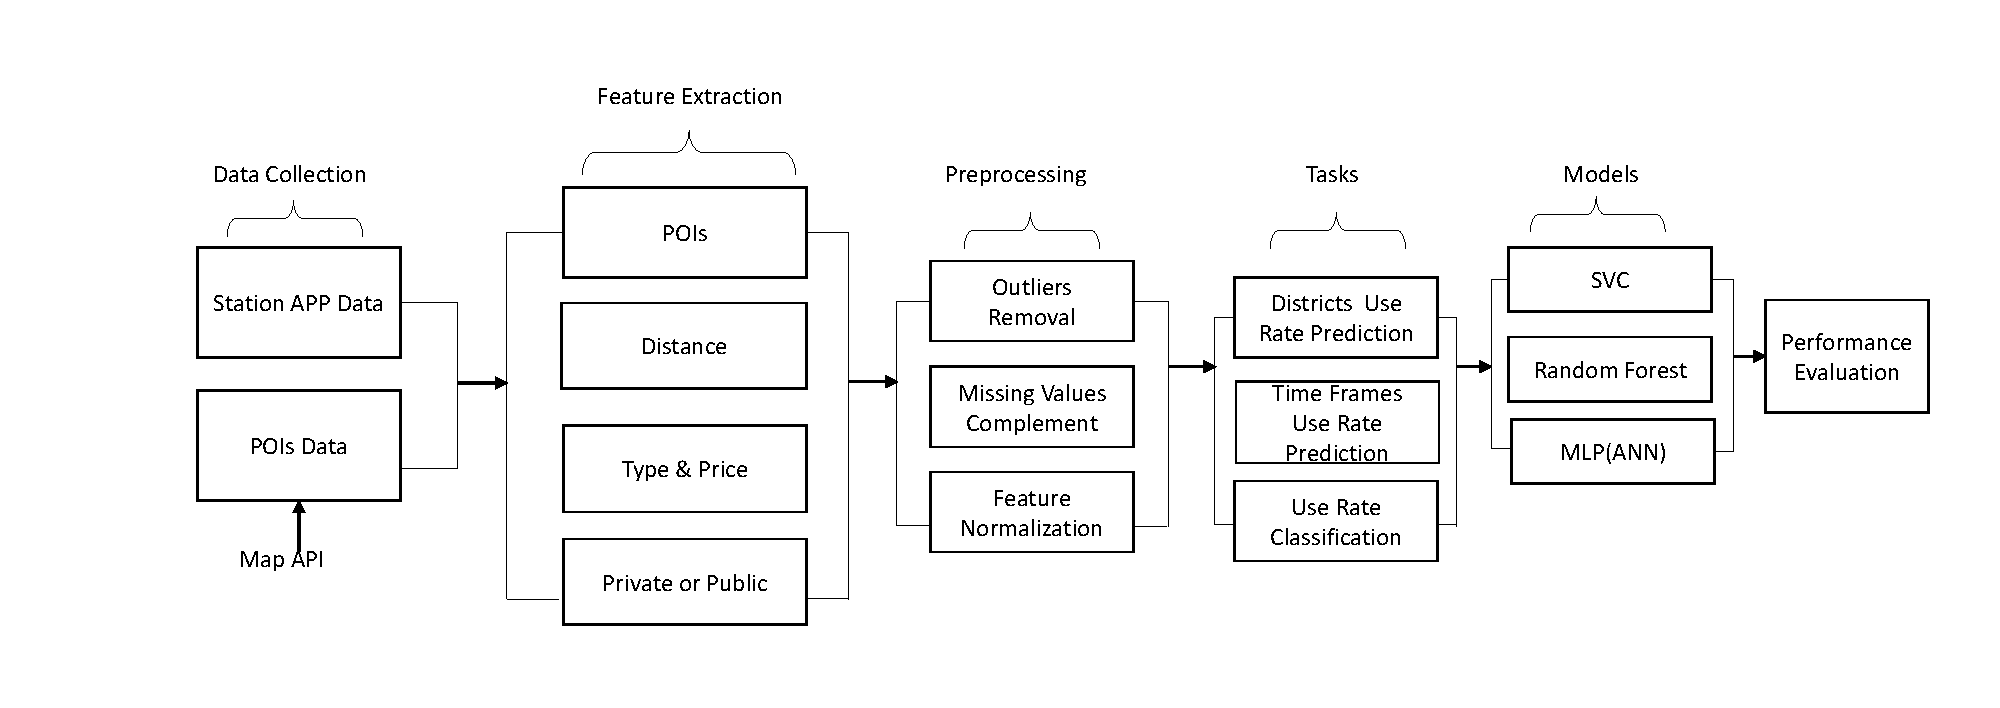
\includegraphics[width=2\columnwidth]{./figures/pipeline.pdf}
	\centering
	\caption{Overall Pipelines of Data Processing and Learning}
	\label{fig2}
\end{figure*}


\section{Methodology}
\subsection{Feature Extraction}

\subsubsection{Datasets}
In this paper, we gather the charging stations logs from all the existing charging station companies who provide their services in Shanghai, with a total of over 2,000,000 lines. The log has a length of one month, from 2018/10 to 2018/11, in which an hourly summarize of each charging station is recorded, showing whether it's occupied or not.

\subsubsection{Hotspots}
From the data we gathered, we made several observations that benefits the features to be included in the model we present. We separate the data into different time frames in order to determine the overall difference among them, since charging network is a dynamic system.
\begin{figure}[!htbp]
	\begin{tabular}{cc}
		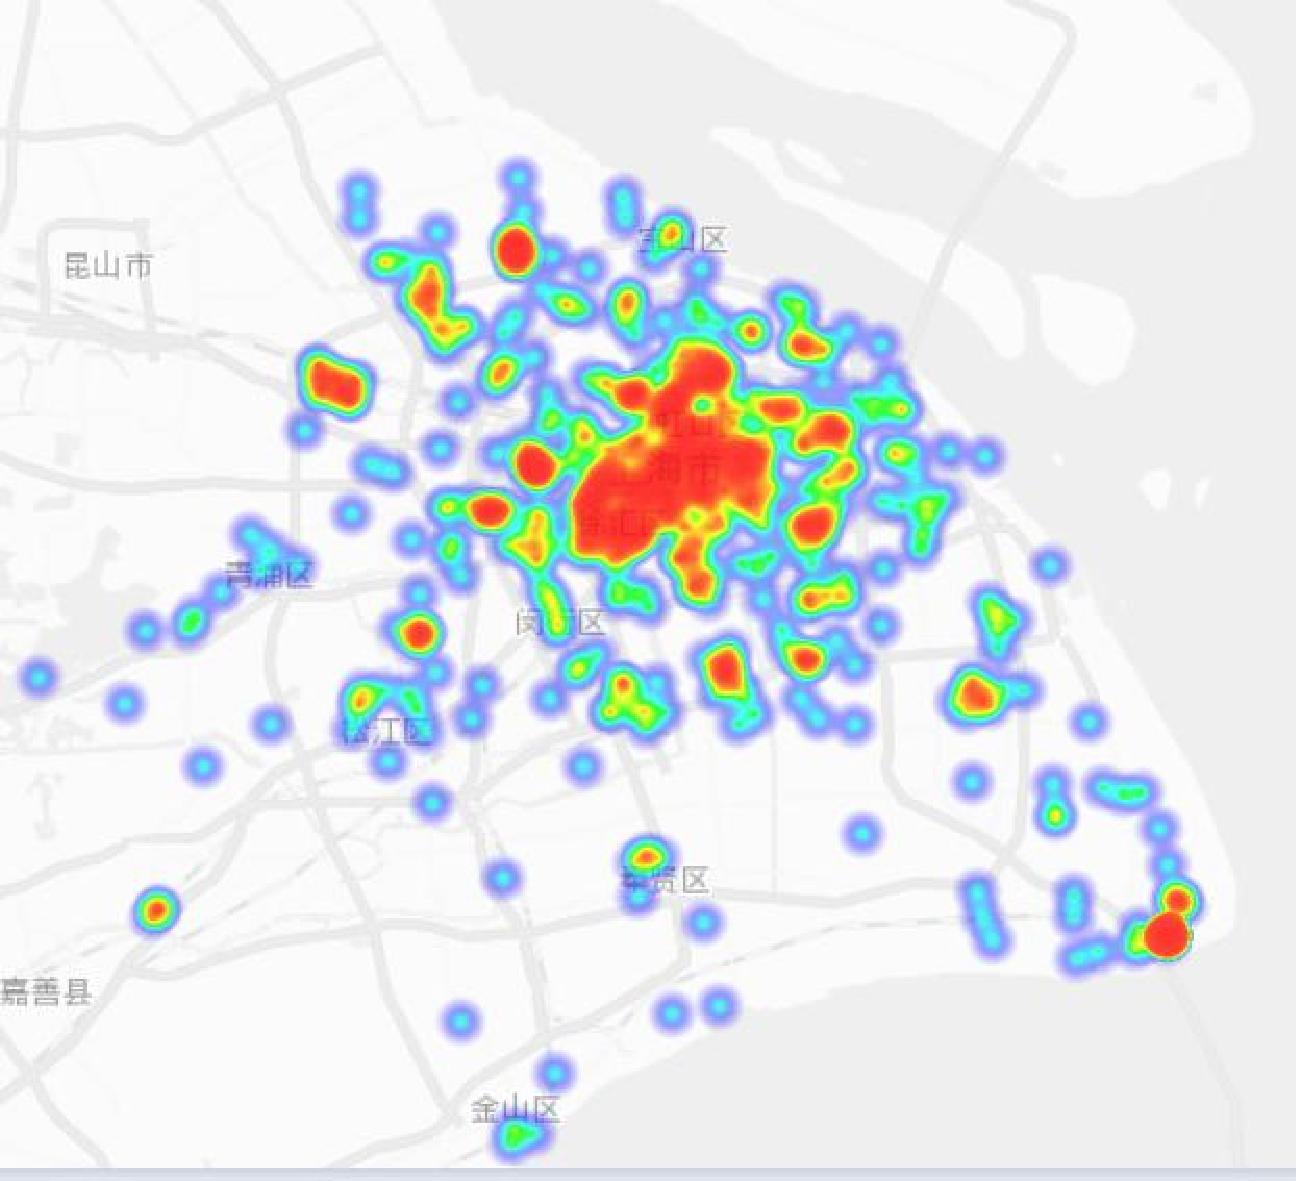
\includegraphics[width=0.45\columnwidth]{./figures/weekday.pdf} &  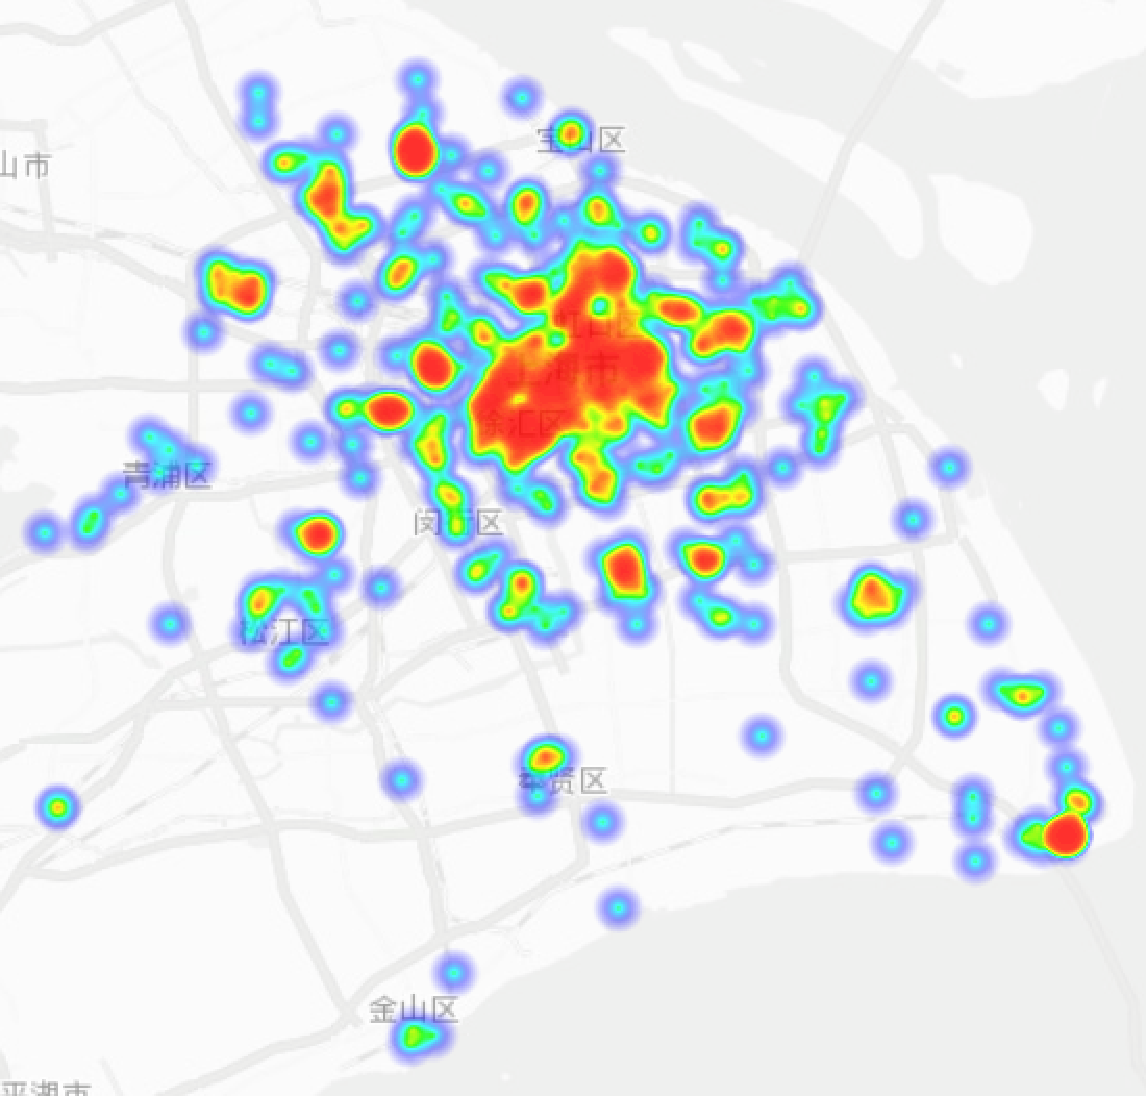
\includegraphics[width=0.45\columnwidth]{./figures/weekend.pdf} \\
		(a) Weekdays & (b) Weekends \\[6pt] 
		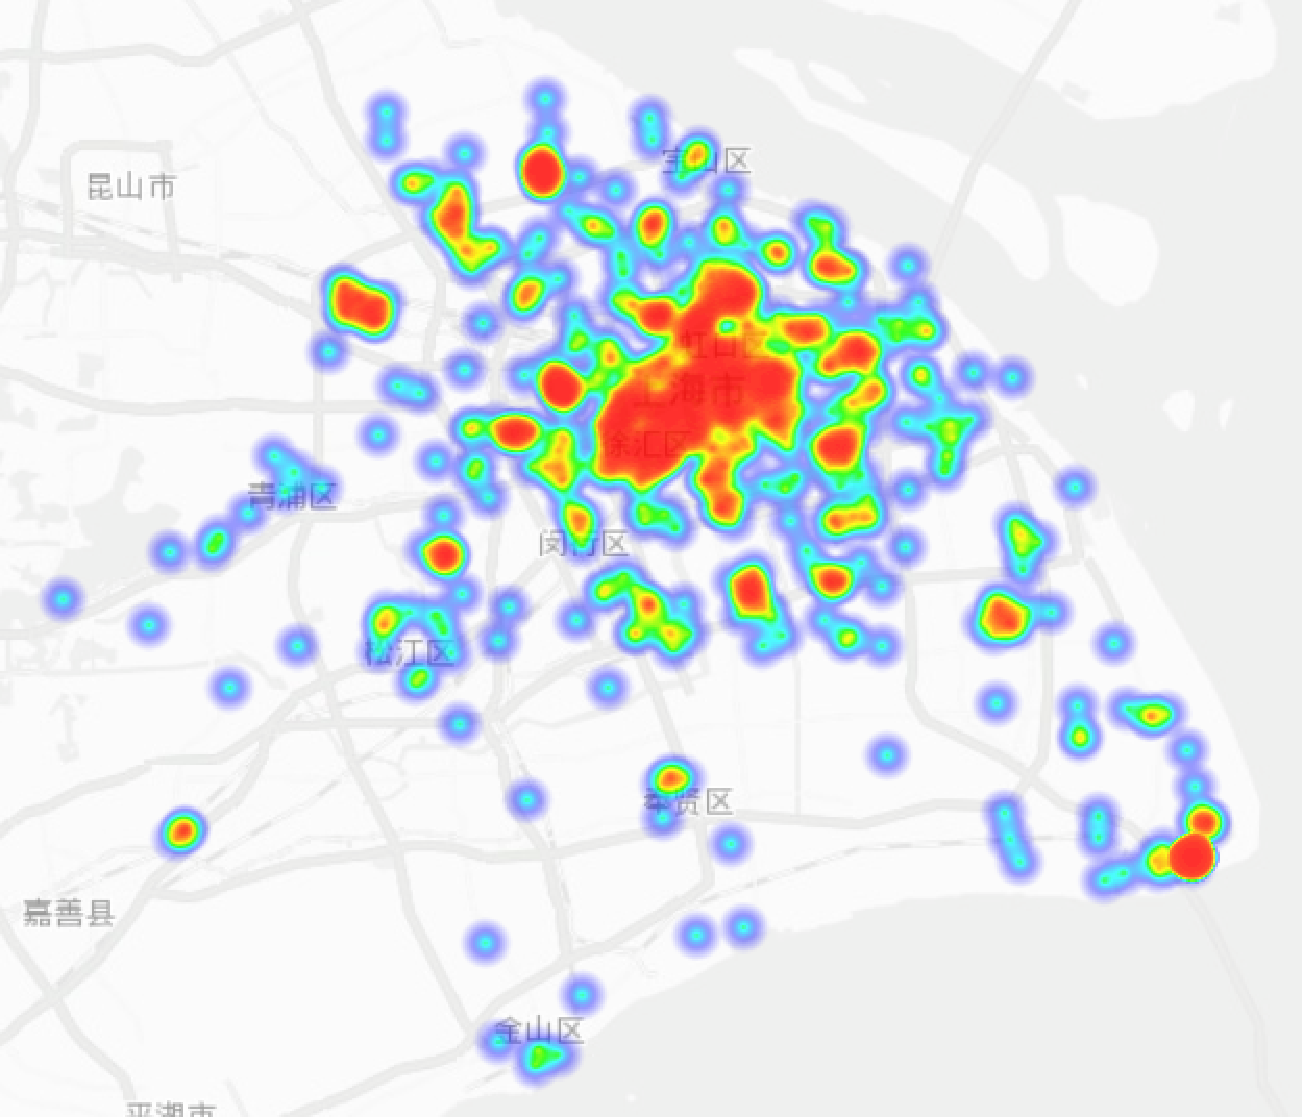
\includegraphics[width=0.45\columnwidth]{./figures/morning.pdf} &
		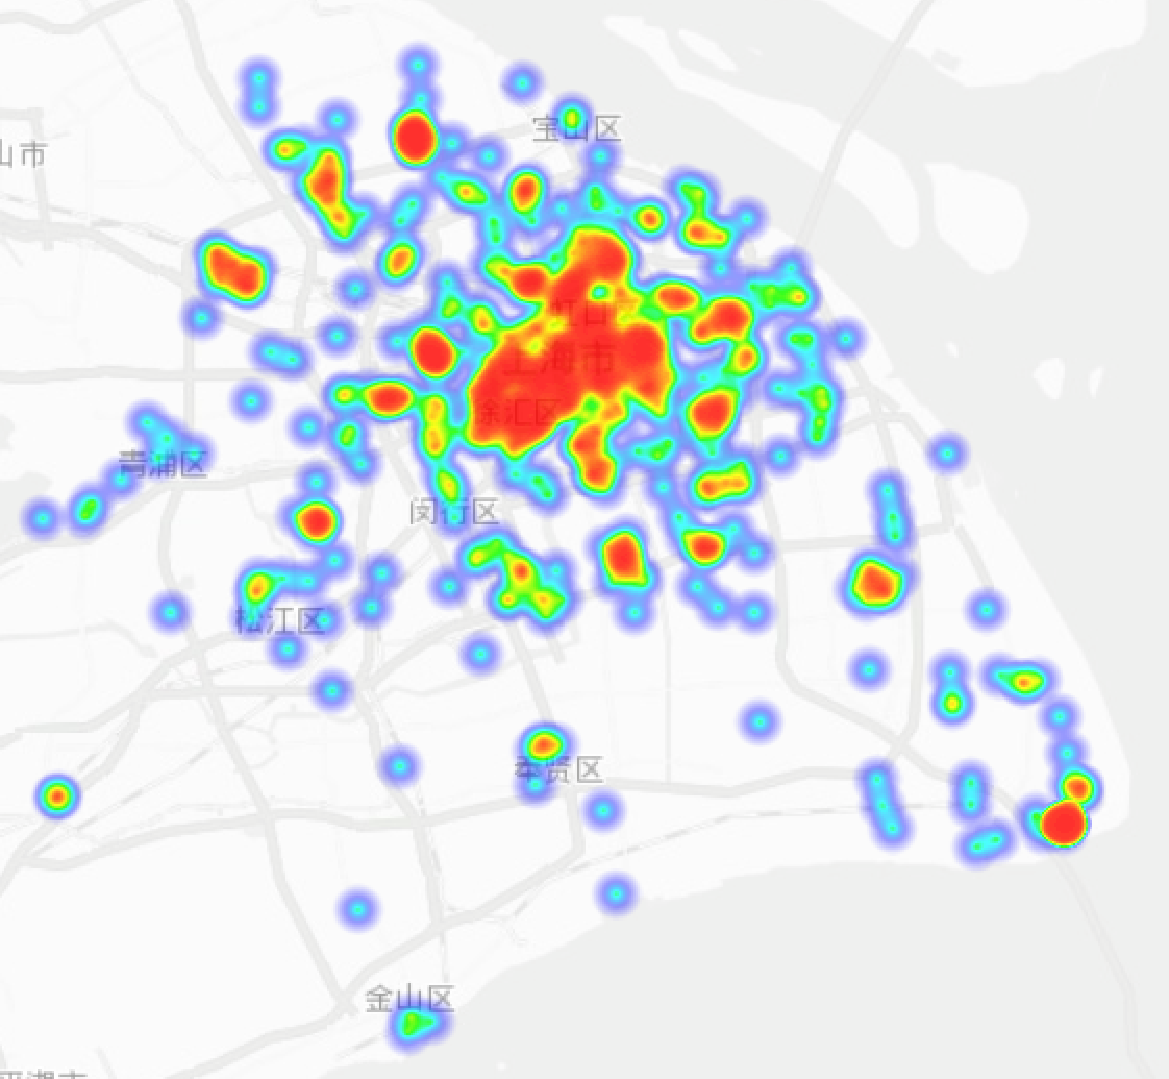
\includegraphics[width=0.45\columnwidth]{./figures/evening.pdf} \\
		(c) Mornings & (d) Evenings
	\end{tabular}
	\centering
	\caption{Charging Hotspots in Shanghai in Different Time Frames}
	\label{fig3}
\end{figure}
From Fig.\ref{fig3}, it is easy to notice that in different time frames, the charging hotspots stays at almost the same locations, meaning that during different time periods, the use rate of a given charging station is determined by its spatiotemporal context.


\subsubsection{Point Of Interest}
To the prosperity of Shanghai, there are so many points of interest(e.g., shopping malls, schools. estates, companies, etc.) located in the city.  Understanding the purpose of the trip by each person who participates in charging system will help us to analyze the use rate prediction. So, we need to extract the POI around each existing charging station. There are a lot of POIs in Shanghai. The POIs are very close to each other. We set a radius around each station and then collect the POIs within the radius. Based on our experiment, choosing a radius as 300 meters is proper. In our work, we get 80 different types of POI totally. Some of the POIs are very similar to each other. Therefore, we group 80 POIs in further step. By grouping POIs, we get 10 groups at last. Table.\ref{tab1} gives the groups and POIs in detail.

\begin{table}[!htbp]
	\caption{Groups of POIs}
	\begin{center}
		\begin{tabular}{|l|p{5cm}|}
			\hline
			Group & Points of interests\\
			\hline
			Food & chinese \& foreign restaurant, snack bar, cake \& dessert shop, cafe, bar\\
			\hline
			Hotels & star hotel, express hotel, apartment hotel\\
			\hline
			Shopping & shopping centers, department stores, supermarkets, convenience stores, home building materials, home appliances digital, shops, markets\\
			\hline
			Education & institutions of higher learning, middle schools, primary schools, kindergartens, adult education, parent-child education, special education schools, study agencies, research institutions, training institutions, libraries, science and technology museums\\
			\hline
			Cultural venue & press and publication, radio and television, art groups, art galleries, exhibition halls, cultural palaces\\
			\hline
			Medical & general hospitals, specialist hospitals, clinics, pharmacies, medical examination institutions, nursing homes, emergency centers, disease control centers\\
			\hline
			Car service & car sales, car repair, car beauty, auto parts, car rental, car inspection field\\
			\hline
			Transportation & airport, railway station, subway station, subway line, long-distance bus station, bus station, bus line, port, parking lot, refueling station, service area, toll station, bridge, charging station, roadside parking space\\
			\hline
			Estates & Office building, residential area, dormitory\\
			\hline
		\end{tabular}
		\label{tab1}
	\end{center}
\end{table}

\subsubsection{Distance}

In use rate prediction, we need to consider distance. People will not choose to park their electric cars for charging if the destination they planned to go is far away. In the system, a station with nearer distance to metro stations, financial centers and major functional buildings would easily be used more often. We select the nearest distance to the following to be the distance we considered as features: company, estate, hospital, metro station, shopping center and university. Fig.\ref{fig4} shows the total count of these important 'distance' POIs, from the figures we can see that these features almost satisfy the long tail distribution, which will be normalized in later work, see Preprocessing part.

\begin{figure}[!htbp]
	\begin{tabular}{cc}
		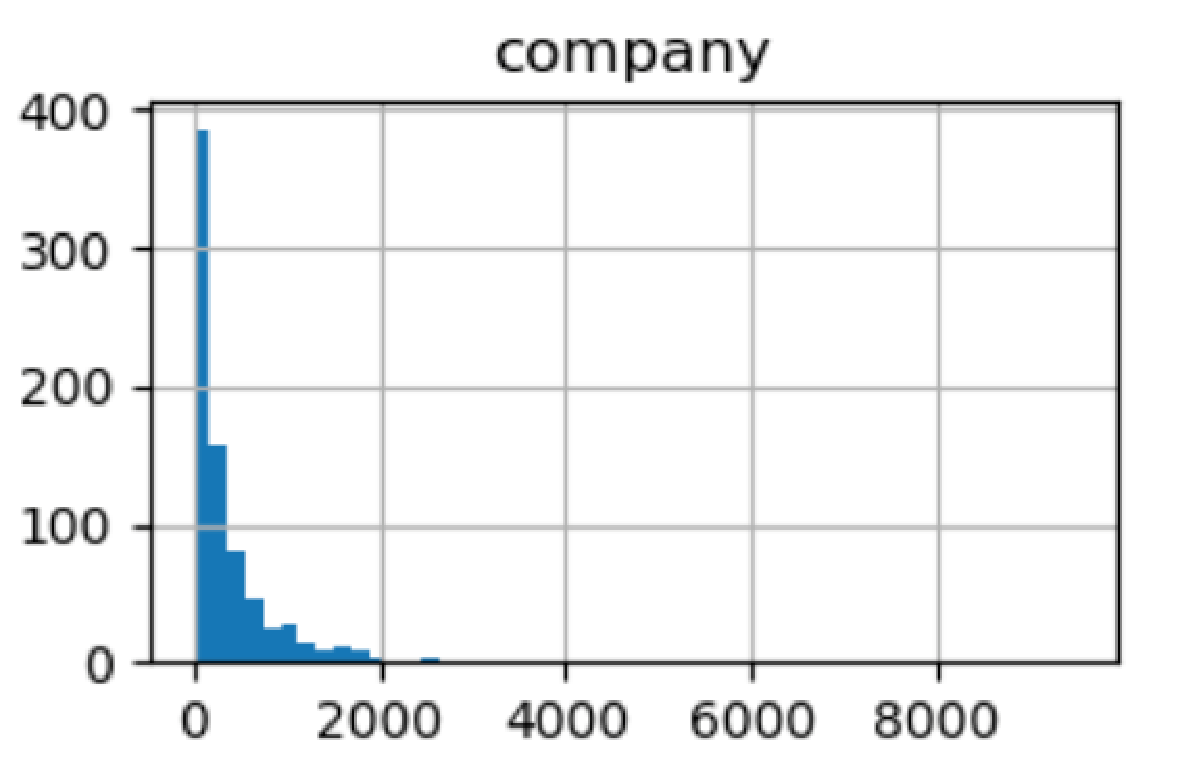
\includegraphics[width=0.45\columnwidth]{./figures/company.pdf} &  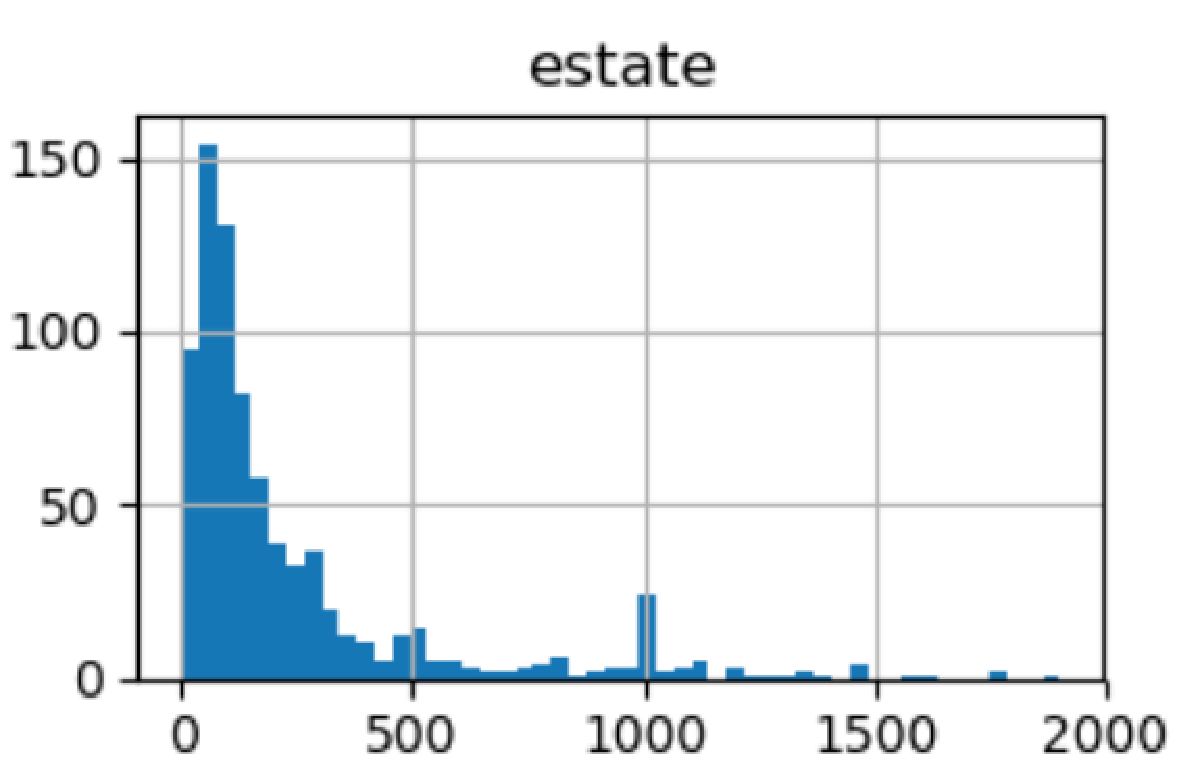
\includegraphics[width=0.45\columnwidth]{./figures/estate.pdf} \\
		(a) Company & (b) Estate \\[6pt] 
		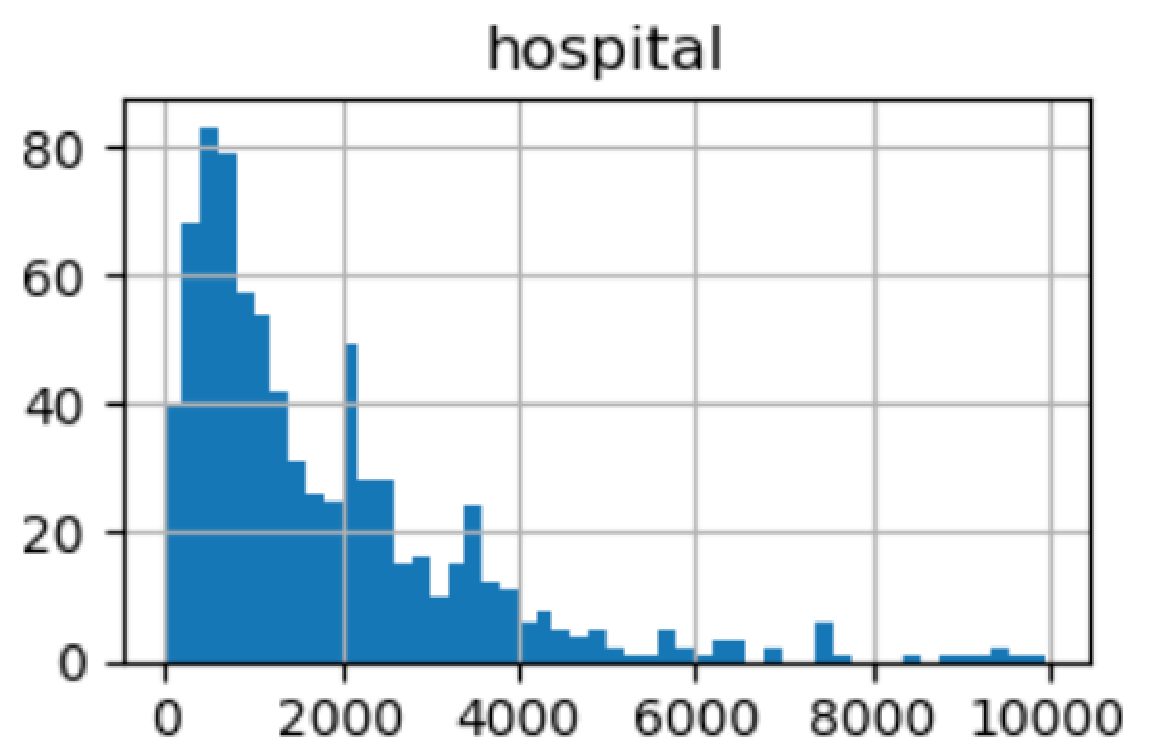
\includegraphics[width=0.45\columnwidth]{./figures/hospital.pdf} &
		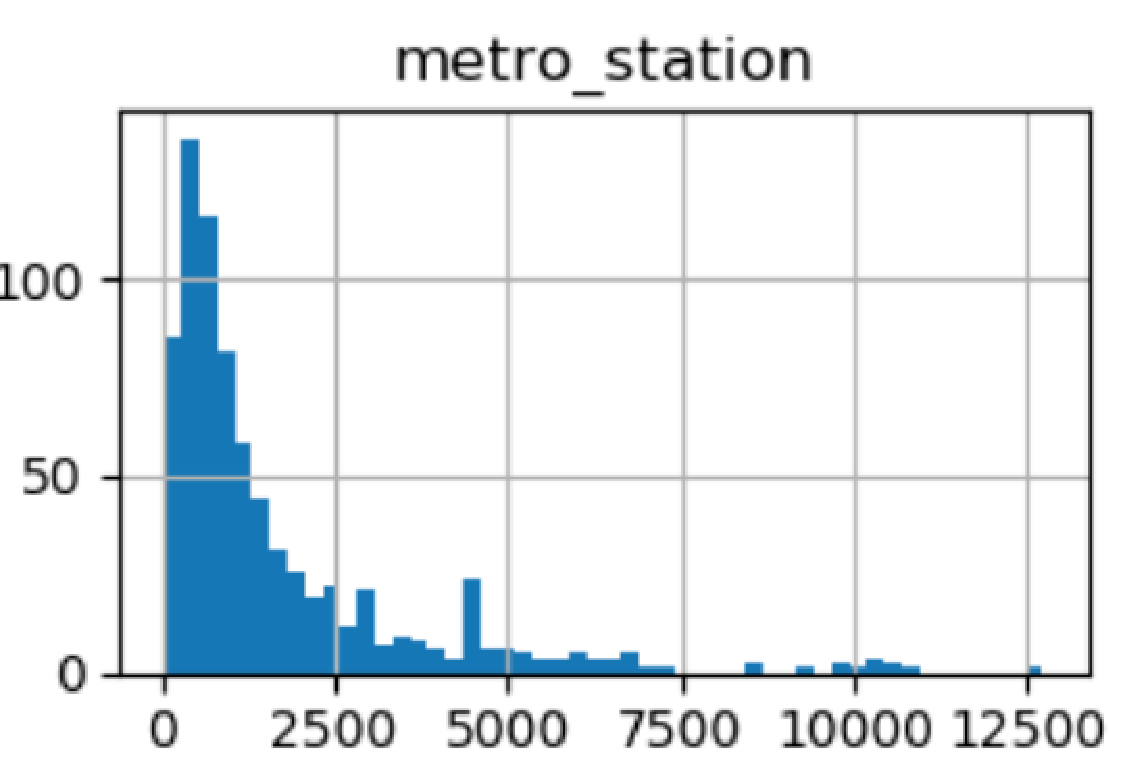
\includegraphics[width=0.45\columnwidth]{./figures/metro.pdf} \\
		(c) Hospital & (d) Metro Station \\
		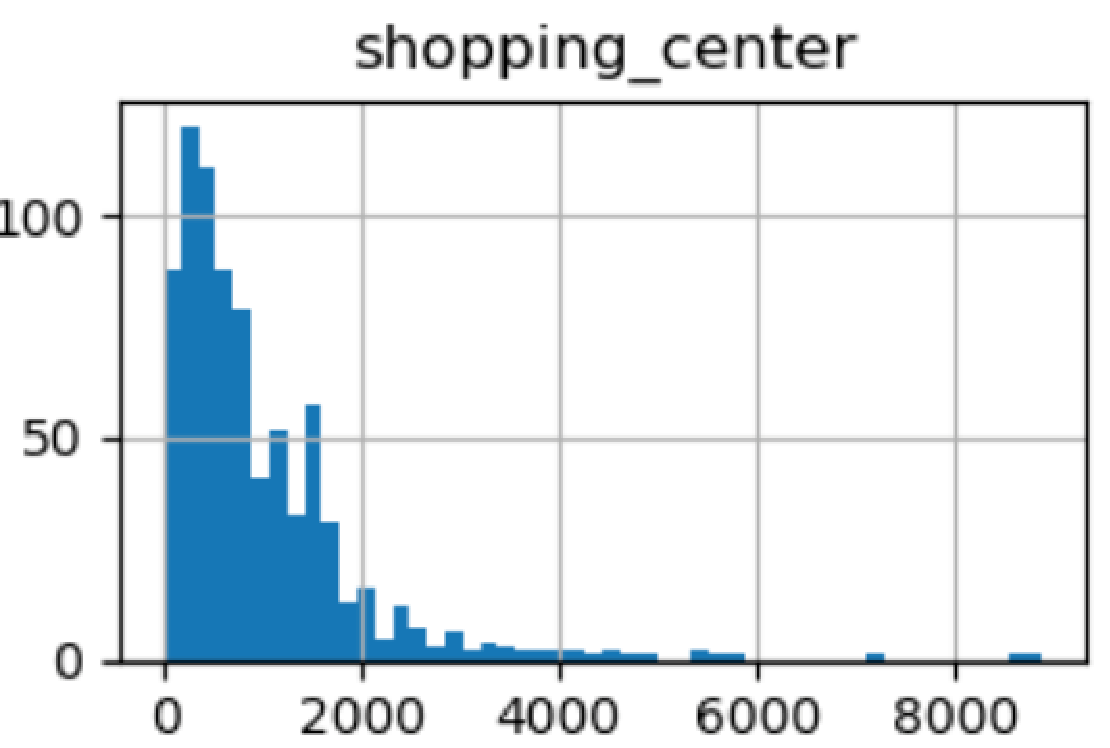
\includegraphics[width=0.45\columnwidth]{./figures/shop.pdf} 
		&
		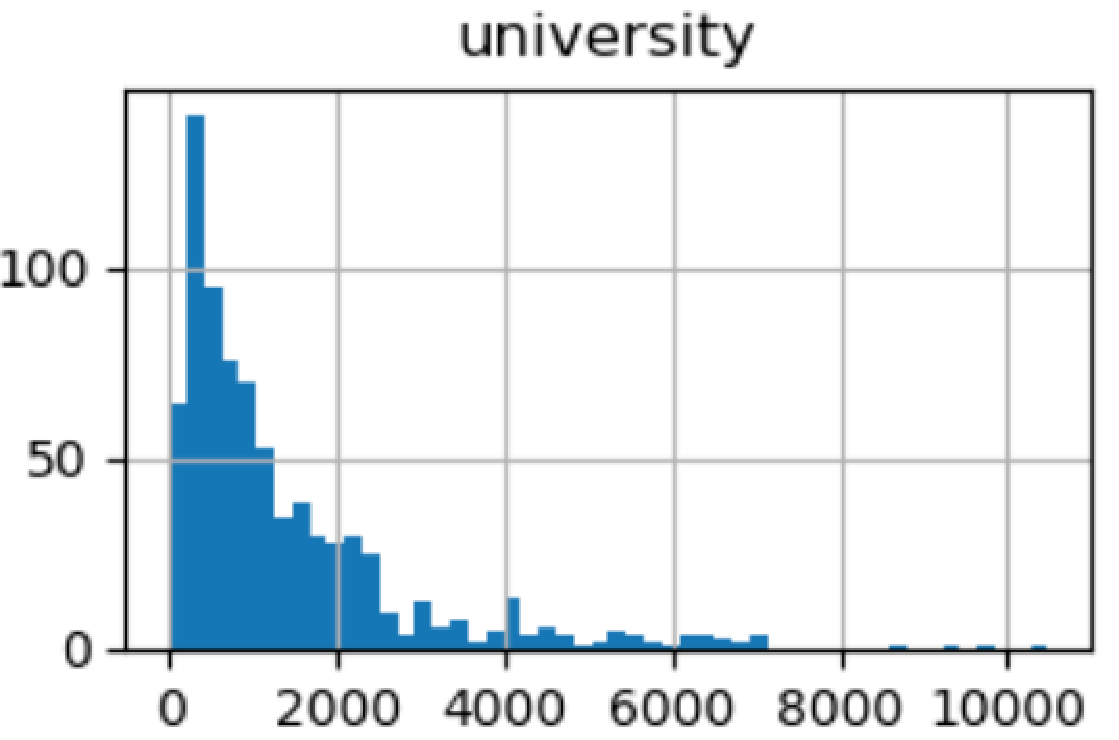
\includegraphics[width=0.45\columnwidth]{./figures/university.pdf} \\
		(e) Shopping Center & (f) University
	\end{tabular}
	\centering
	\caption{Count of Important POIs}
	\label{fig4}
\end{figure}

\subsubsection{Type \& Price}
By futher digging into the data, we find that there is a 0.3 correlation between price for charging and the use rate. Since there are two types of charging ports: DC and AC. We would include the number of ports and the price of both types in a charging station as one of its feature. Fig.\ref{fig5} shows the number of AC/DC type of stations's charging ports, as well as each type's charging cost fee. From the figures we observe that there are much more AC type charging ports than DC type ones, while the charging cost fee of them two are almost the same.

\begin{figure}[!htbp]
	\begin{tabular}{cc}
		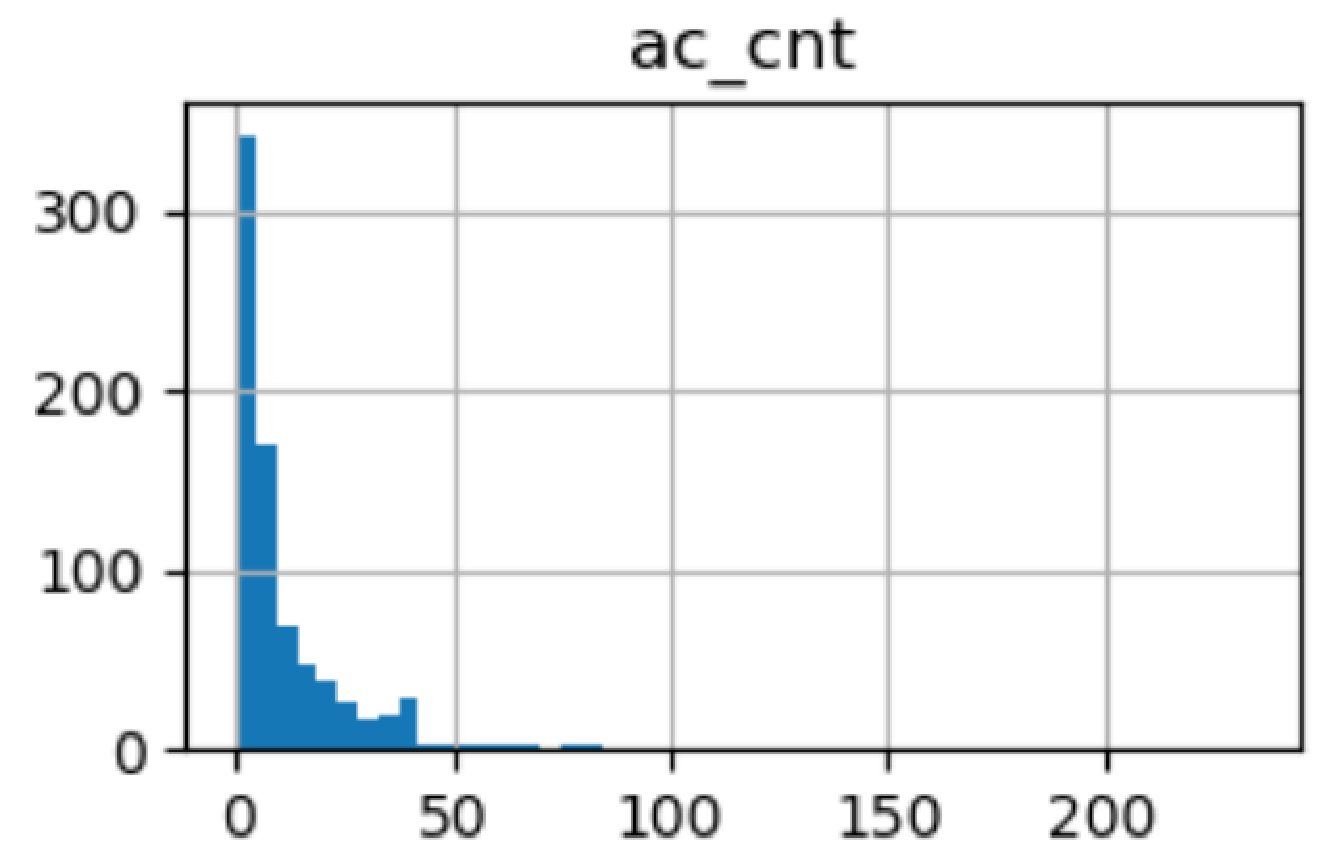
\includegraphics[width=0.45\columnwidth]{./figures/ac_cnt.pdf} &  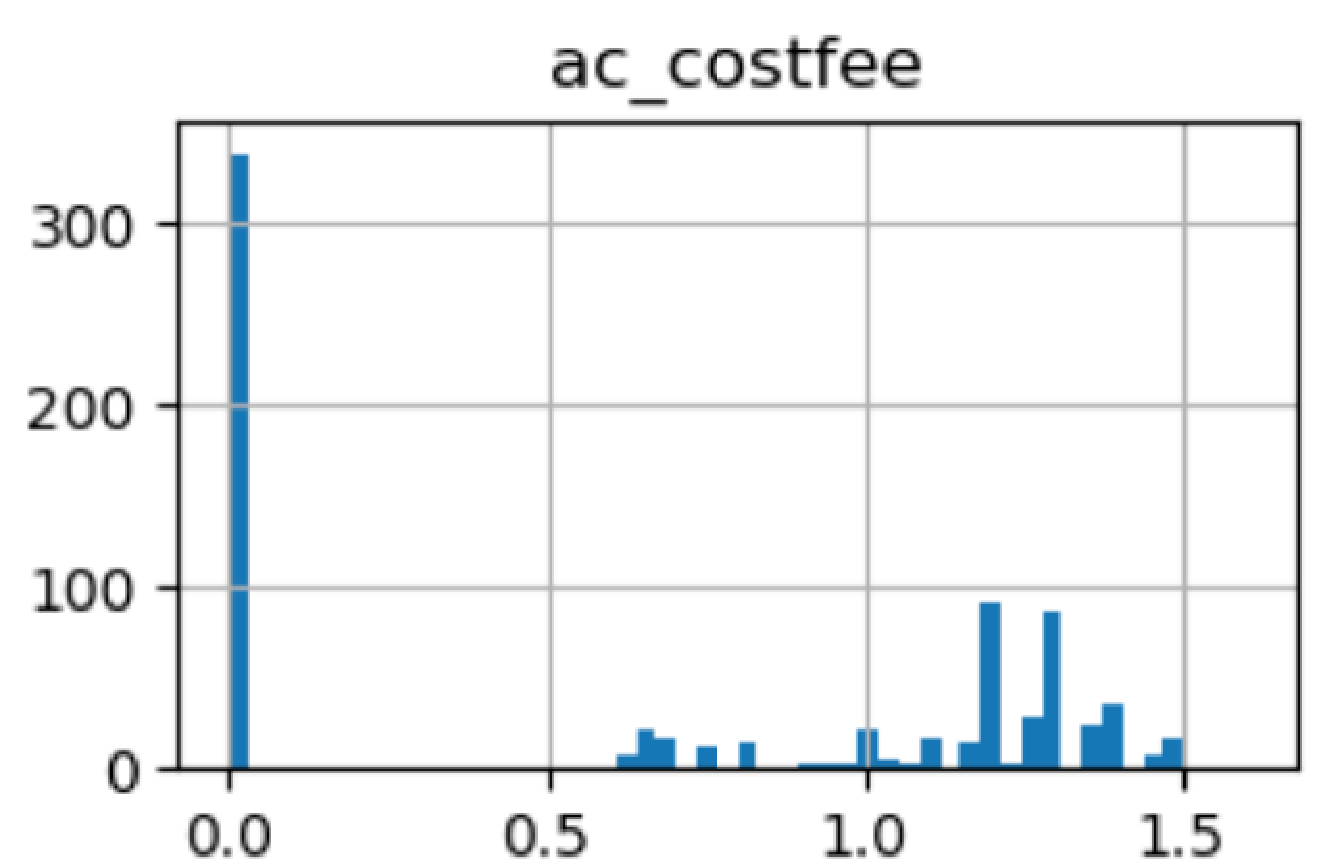
\includegraphics[width=0.45\columnwidth]{./figures/ac_fee.pdf} \\
		(a) AC\_Count & (b) AC\_Fee \\[6pt] 
		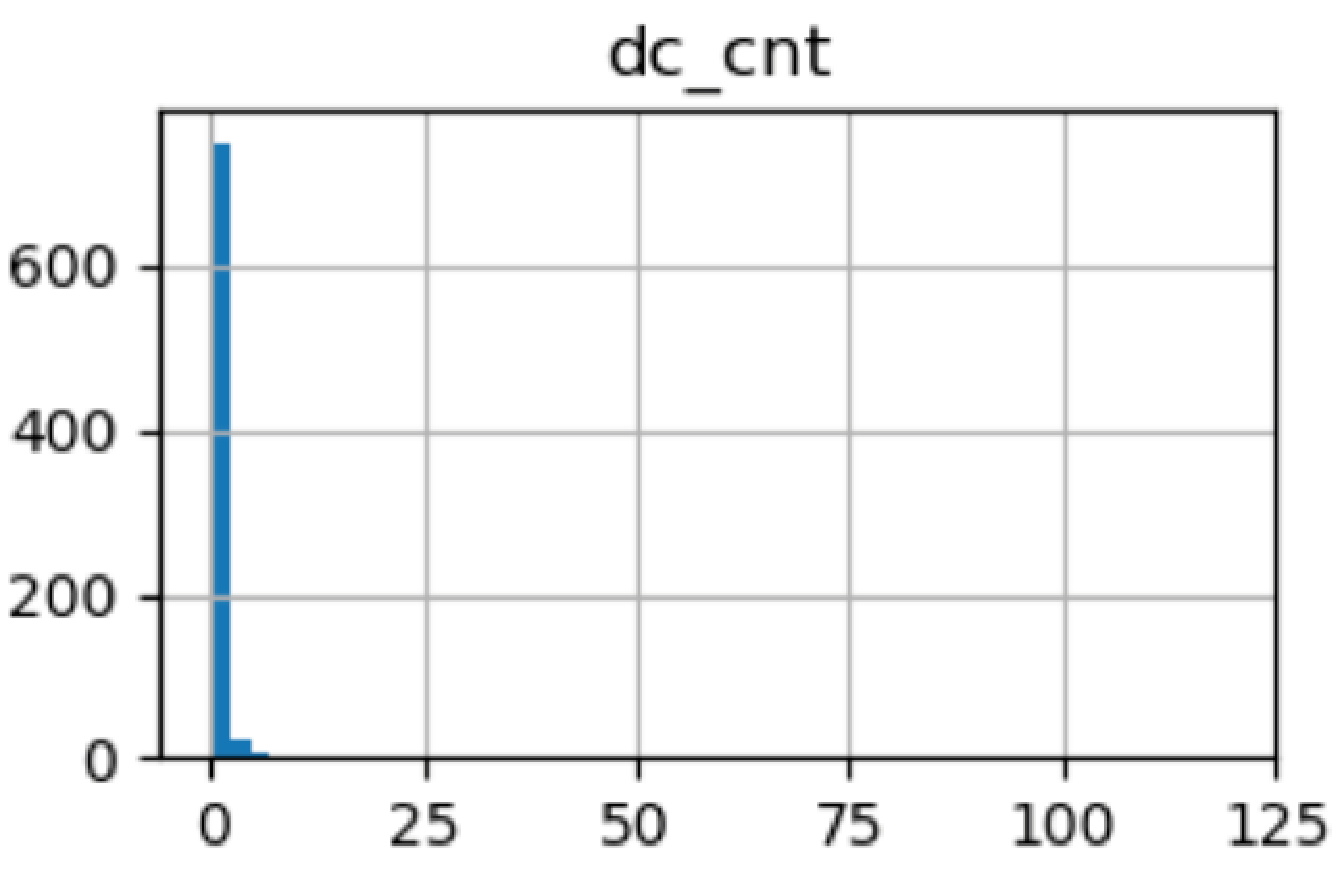
\includegraphics[width=0.45\columnwidth]{./figures/dc_cnt.pdf} &
		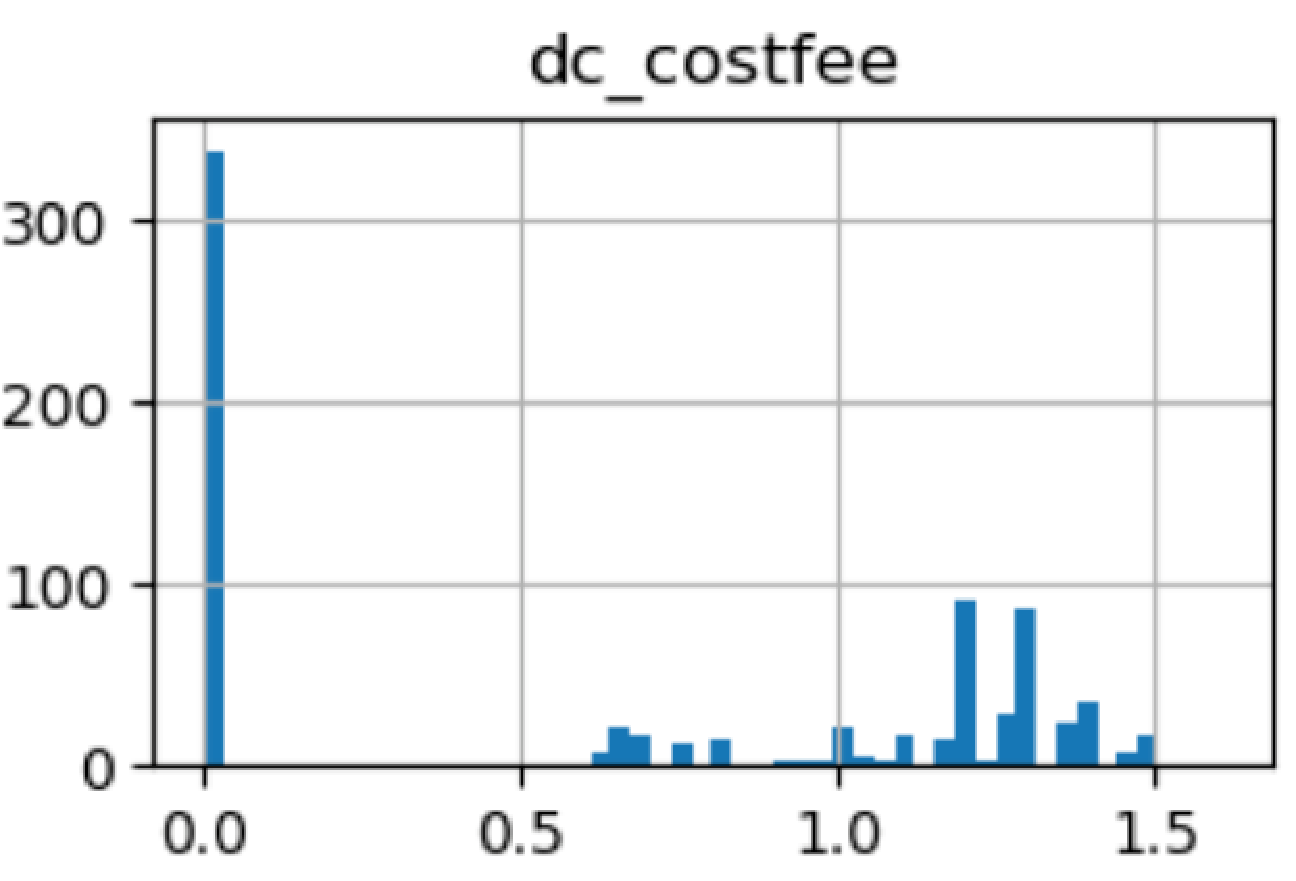
\includegraphics[width=0.45\columnwidth]{./figures/dc_fee.pdf} \\
		(c) DC\_Count & (d) DC\_Fee
	\end{tabular}
	\centering
	\caption{Charging Stations Types and Charging Cost Fee}
	\label{fig5}
\end{figure}

\subsubsection{Private or public}
By observing the data we've collected, it can be seen that most of the charging stations are private charging stations, which means they are typically used by electric buses and rent cars, or used by specific companies for their employees, accounting for over 70\% of the total charging stations. Also, since the private are used by more regular users(e.g., buses, companies employees), its use rate are 5\% higher compared to public ones. This alongside other observations will be taken into consideration.

\subsection{Spatio Temporal Data Based Framework}

\subsubsection{Ditricts}
There are 16 districts of station data in total, Fig.\ref{fig6} shows the distribution of charging stations in Shanghai. And for experiment , we separate them into two parts as urban area and suburb area. The final dataset for district prediction task contains the two parts of data, in urban part, 7 districts are included while in suburb part, 9 left districts are included.
\begin{figure}[!htp]
	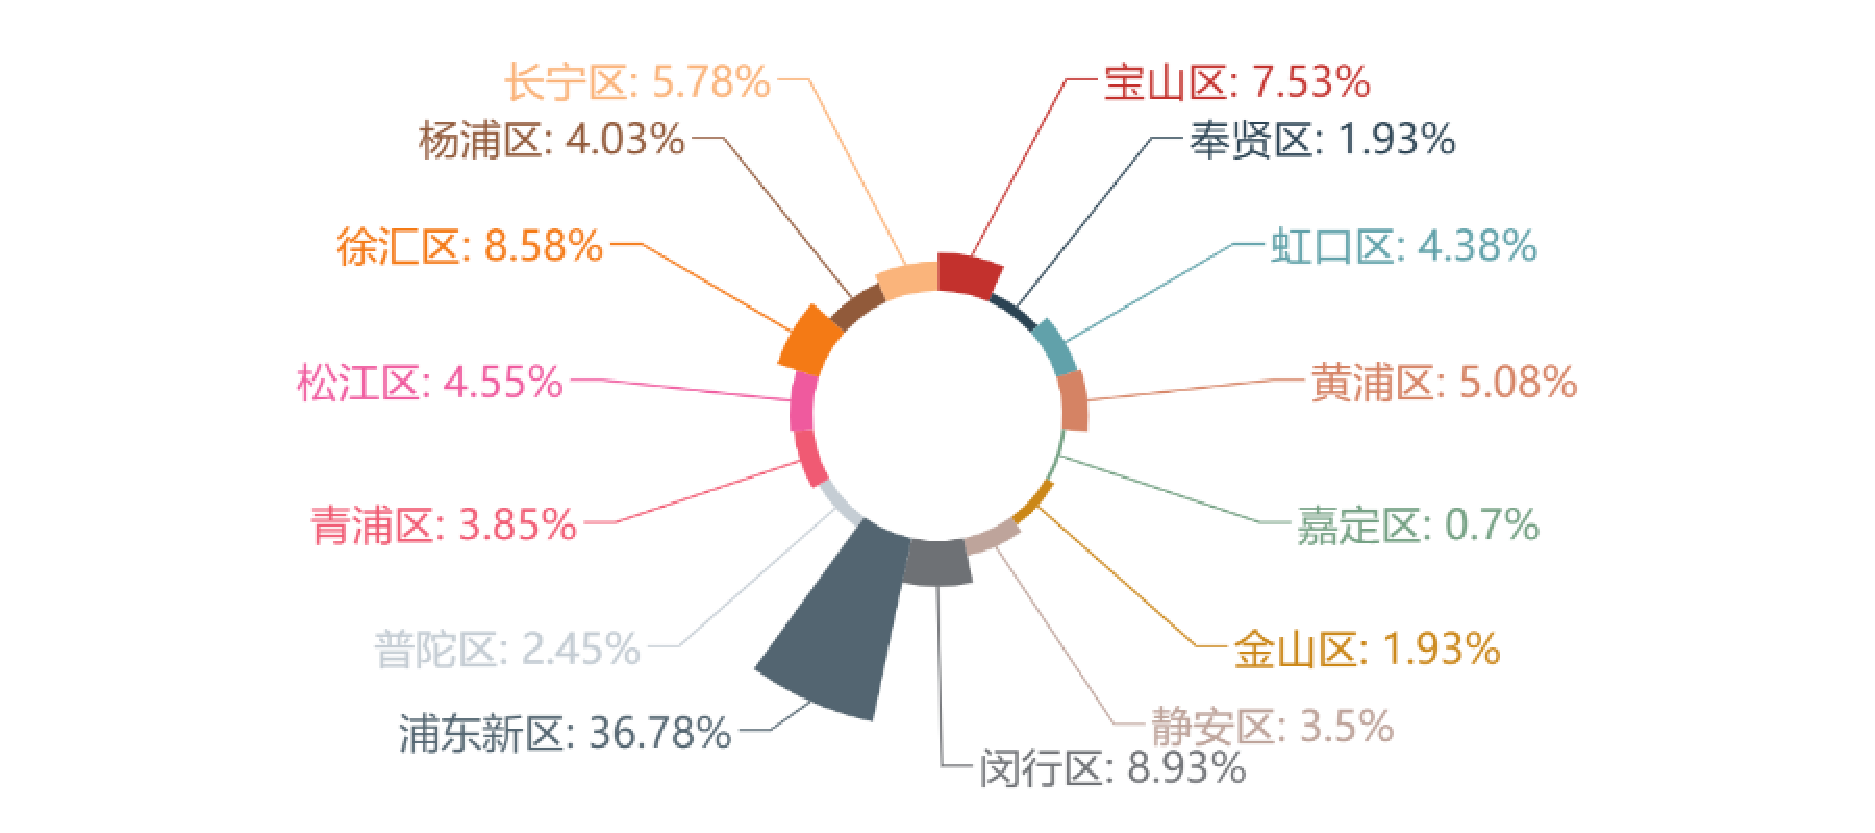
\includegraphics[width=\columnwidth]{./figures/distribution.pdf}
	\centering
	\caption{District Distribution of Charging Stations}
	\label{fig6}
\end{figure}
\subsubsection{Time Frames}
In order to further study stations' use rate in different time periods, we set different time frames, including total time, weekday, weekend, daytime, evening time, morning\_rush hours, evening\_rush hours and travel\_hours, to help observe the use rate discrepancy during these phases. Fig.\ref{fig7} shows the average use-rate of the time frames above.
\begin{figure}[!htp]
	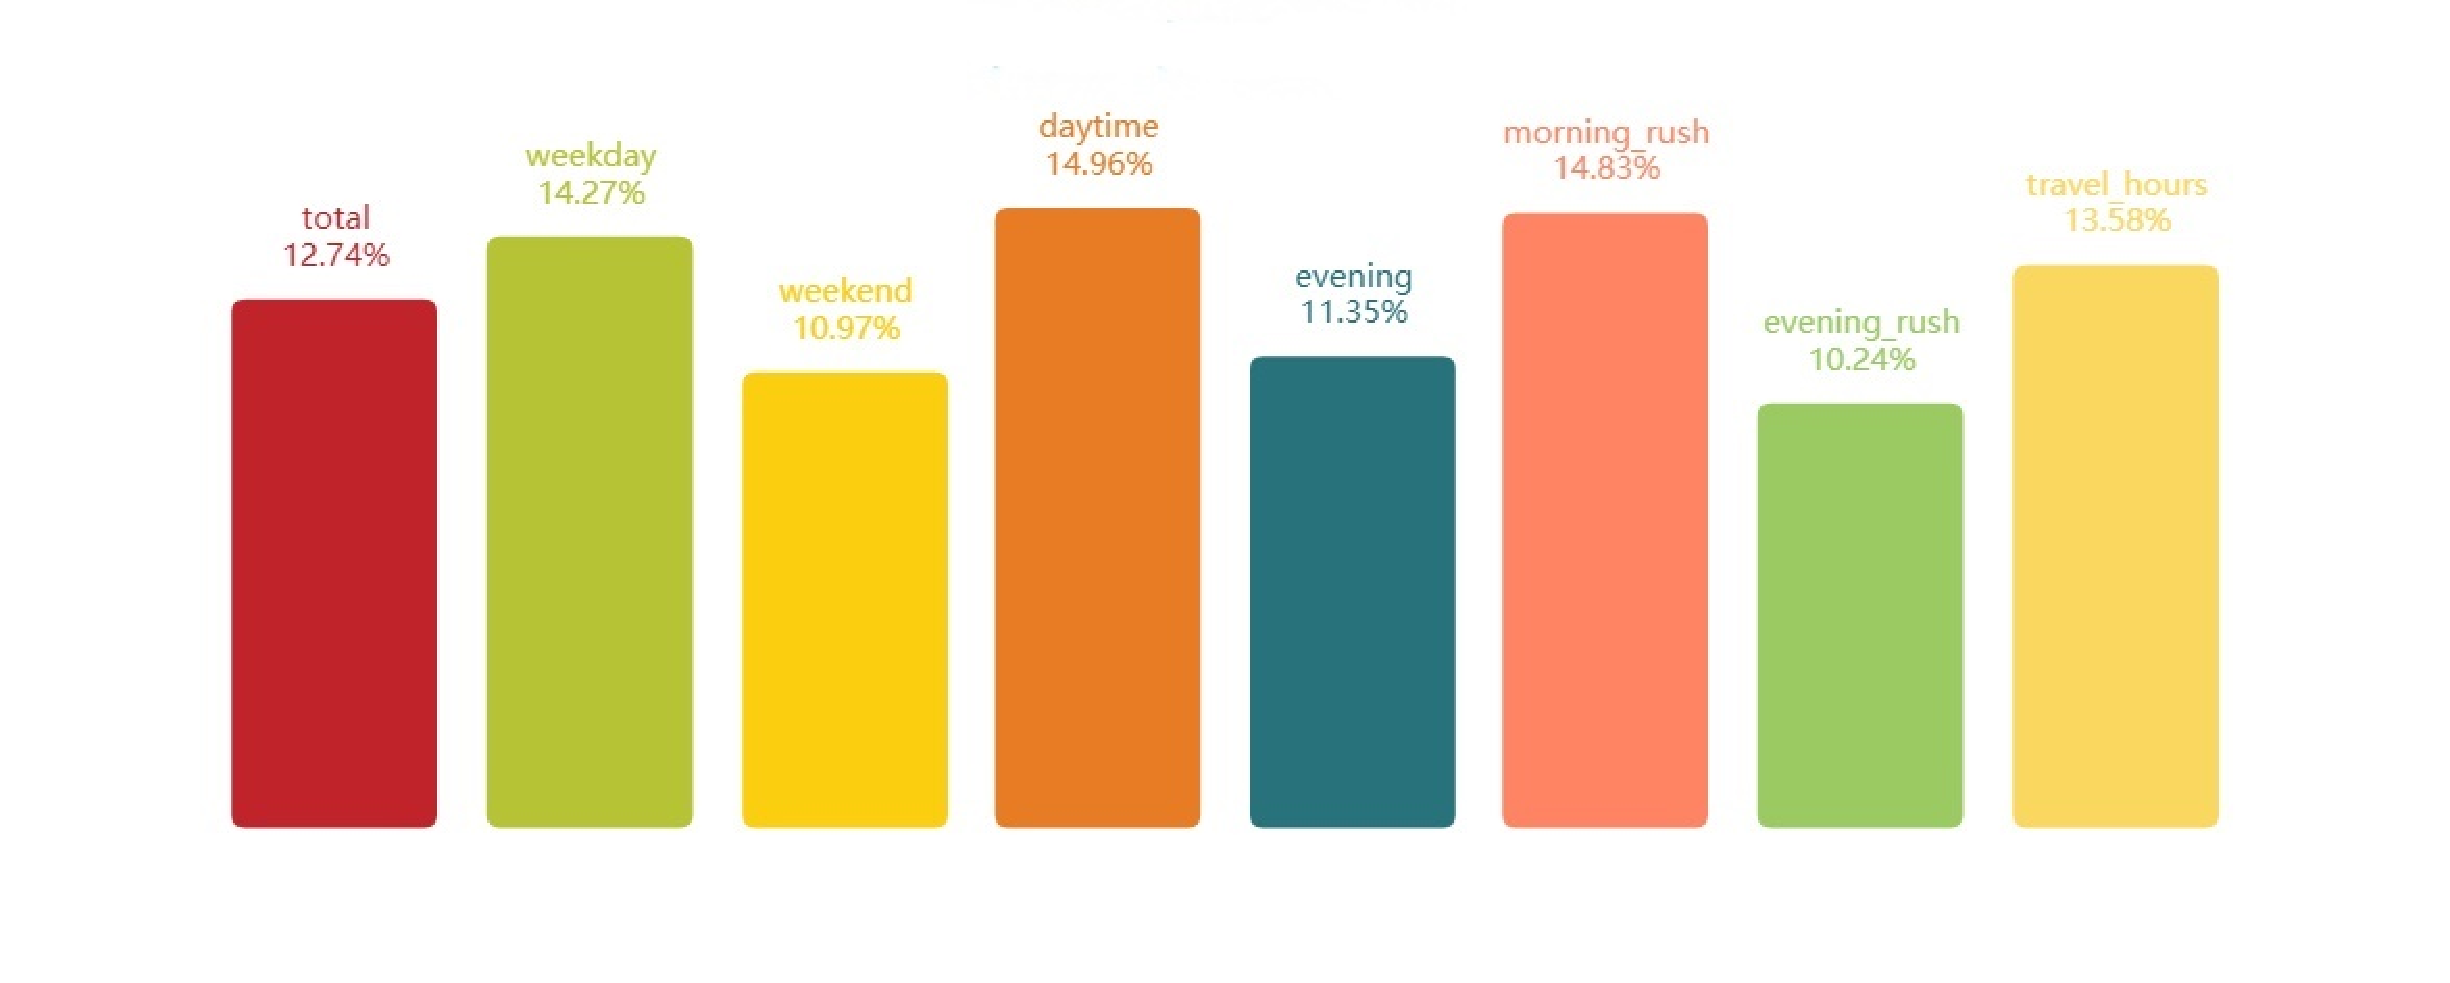
\includegraphics[width=\columnwidth]{./figures/timeframes.pdf}
	\centering
	\caption{Average Use Rate in Different Time Frames}
	\label{fig7}
\end{figure}

\subsection{Preprocessing}
\subsubsection{Data Cleaning}
The original dataset may exist some outliers and missing values, there should be a data cleaning procedure to deal with these invalid data. For outliers, if detected, we remove them from the dataset; for missing values, we use the median filling method to fill blanks with median values computed via 'Imputer' function.

\subsubsection{Feature Zooming}
In 'nearest important POIs', the value of each feature is over hundred, while in other features like 'dc cost fee', the mean value is just about 0.85 per hour. In order to achieve a better performance using machine learning algorithms, we take a feature zooming procedure to normalize feature values so that they can range in [0,1]. Different models may use different zooming strategies, which will be discussed in detail in experiment section. Fig.\ref{fig8} shows an example of the feature 'university' after normalization step.
\begin{figure}[!htp]
	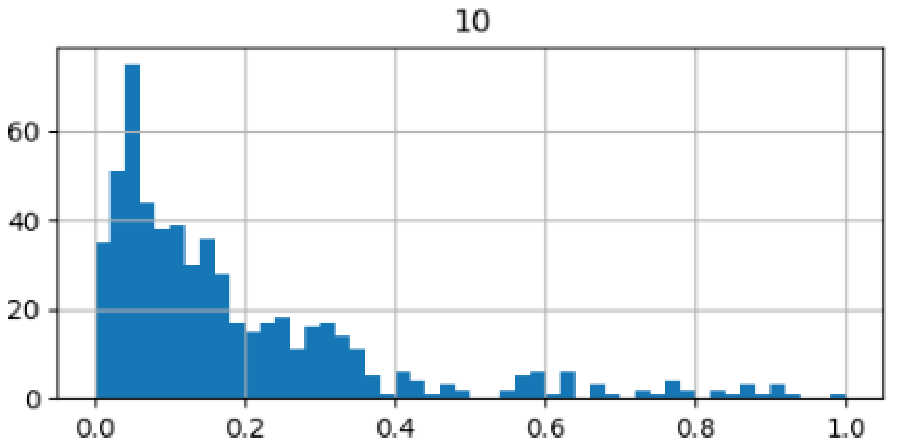
\includegraphics[width=\columnwidth]{./figures/uni.pdf}
	\centering
	\caption{An Example of Feature Normalization}
	\label{fig8}
\end{figure}
\subsection{Implementation}
We aim to implement that when given important features, the model can tell what's the level of a station's use rate. Because the use rate of charging stations range in [0,1), so we set three levels as labels for classification task. In detail, we set use rate from 0 to 20\% as low\_use\_rate; 20\% to 50\% as mid\_use\_rate; and over 50\% as high\_use\_rate. For prediction tasks in both districts dataset and time frames dataset, we take features including stations' surrounding POIs, the number of nearest important POIs(e.g., company, estate, hospital, metro station, shopping center, university), charging port type, charging cost fee and whether it's for private or public use, into consideration. Then we make use of three classification models: SVC, Random Forest and MLP(ANN). With features added into these models, we evaluate the final results and find relationships between classification accuracy and features. The detailed experiment procedure will be discussed in next section.


\section{Experiments}
\subsection{Parameter Settings}
We run our dataset on SVM, Random Forest and MLP respectively. For SVM, we make use of its 'SVC' module for classification task and choose 'linear' function for its kernel, the punishment parameter C is set to default as 1.0. For Random Forest, we set the number of decision-making trees 'n\_estimators' as 8. For MLP, we choose 'lbfgs' as solver and the activation function is 'relu', in order to avoid overfitting, we set the regular term alpha as 1e-4, the hidden\_layer\_sizes is set to (5,3) to achieve the best performance.

\subsection{District Prediction}
The task of district prediction aims to classify stations into high, middle or low use rate in urban and suburb areas of Shanghai.

We first separate our dataset into two parts: urban areas data and suburb areas data. After this operation, about 30\% of station data is in the urban one, and other 70\% of data is in the suburb one. Then, for each part, we randomly choose 80\% of the data as training set, and 20\% left as test set. For SVC and MLP, there shoule be a feature normalization procedure, we conduct MinMaxScaler for SVC and StandarScaler for MLP to set constraints on feature value so that they can range in (0,1). For Random Forest, there's no need for normalization, so we keep the feature data as original when we implement our experiment on it. We use mean average precision(MAP) as evaluation method which is commonly used in multilabel classification task.

Table.\ref{tab2} and Table.\ref{tab3} show the prediction accuracy of different models on urban areas data and suburb areas data. From the results we observe that: (1) SVC and Random Forest can perform stably on both two tasks. (2) MLP performs best in suburb prediciton while performs worst in urban prediction. The reason we infer is that because of the distribution of station data mentioned above, the urban part has lower data volume than the suburb part, this may influence the model performance due to MLP's neural network characteristic, while SVC and Random Forest are not sensitive to this difference.
\begin{table}[htbp]
	\caption{Evaluation results on urban prediction}
	\begin{center}
		\begin{tabular}{|l|l|}
			\hline
			Model & Accuracy\\
			\hline
			LR & 60.9\%\\
			\hline
			SVM & 68.9\%\\
			\hline
			Random Forest & 70.1\%\\
			\hline
			XGBOOST & 73.6\%\\
			SVC & 84.62\%\\
			\hline
			MLP & 74.35\%\\
			\hline
			Random Forest & 79.52\%\\
			\hline
			(Mean) & 79.50\%\\
			\hline
		\end{tabular}
		\label{tab2}
	\end{center}
\end{table}
Table.\ref{tab2} shows the prediction accuracy of different models. We can see that they can all perform well based on our settings, and XGBOOST achieves the most favourable result.

\begin{table}[htbp]
	\caption{Evaluation results on suburb prediction}
	\begin{center}
		\begin{tabular}{|l|l|}
			\hline
			Model & Accuracy\\
			\hline
			SVC & 79.52\%\\
			\hline
			MLP & 80.72\%\\
			\hline
			Random Forest & 78.31\%\\
			\hline
			(Mean) & 79.52\%\\
			\hline
		\end{tabular}
		\label{tab3}
	\end{center}
\end{table}

\subsection{Time Frames Prediction}
Stations' use rate in different time frames is a more concerned problem we want to explore. According to time frames partition mentioned in Section 4, we also separate station data into 7 time frames: weekday, weekend, morining, morning\_rush\_hours, evening, evening\_rush\_hours and travel hours. In this task, features like POIs, charging port type and charging price still stay the same, while the use rate itself will vary in different time frames, so that the level of use rate, also the classification labels will differ from each time frame dataset. After preprocessing, we also randomly choose 80\% of valid data as training set, and the left as test set. We use the same models as used in districts prediction task, SVC, Random Forest and MLP(ANN), and then conduct our experiments.

Table.\ref{tab4} and Table.\ref{tab5} show the accuracy of different models on weekday data and weekend data. We can see that in weekday time, all the three model just perform ordinarily, achieve an average accuracy of 74.71\%. However, in weekend time, all of them perform pretty well and achive a more than 90\% score. We assume that classification models can perform better in a shoter time span dataset. And we continue the further experiments.
\begin{table}[htbp]
	\caption{Evaluation results on weekday prediction}
	\begin{center}
		\begin{tabular}{|l|l|}
			\hline
			Model & Accuracy\\
			\hline
			SVC & 75\%\\
			\hline
			MLP & 76.72\%\\
			\hline
			Random Forest & 72.41\%\\
			\hline
			(Mean) & 74.71\%\\
			\hline
		\end{tabular}
		\label{tab4}
	\end{center}
\end{table}

\begin{table}[htbp]
	\caption{Evaluation results on weekend prediction}
	\begin{center}
		\begin{tabular}{|l|l|}
			\hline
			Model & Accuracy\\
			\hline
			SVC & 96.55\%\\
			\hline
			MLP & 99.13\%\\
			\hline
			Random Forest & 98.27\%\\
			\hline
			(Mean) & 97.98\%\\
			\hline
		\end{tabular}
		\label{tab5}
	\end{center}
\end{table}

Then, we conduct experiments in morning, morning\_rush\_hours, evening, evening\_rush\_hours datasets respectively to verify our assumption. Table.\ref{tab6} and Table.\ref{tab7} show the results on the former two datasets. As the result shows, models perform much better in rush\_hours which has a shorter time span.
\begin{table}[htbp]
	\caption{Evaluation results on morning prediction}
	\begin{center}
		\begin{tabular}{|l|l|}
			\hline
			Model & Accuracy\\
			\hline
			SVC & 75\%\\
			\hline
			MLP & 77.59\%\\
			\hline
			Random Forest & 74.14\%\\
			\hline
			(Mean) & 75.58\%\\
			\hline
		\end{tabular}
		\label{tab6}
	\end{center}
\end{table}

\begin{table}[htbp]
	\caption{Evaluation results on morining\_rush\_hours prediction}
	\begin{center}
		\begin{tabular}{|l|l|}
			\hline
			Model & Accuracy\\
			\hline
			SVC & 95.69\%\\
			\hline
			MLP & 95.69\%\\
			\hline
			Random Forest & 96.55\%\\
			\hline
			(Mean) & 95.98\%\\
			\hline
		\end{tabular}
		\label{tab7}
	\end{center}
\end{table}
The results on evening and evening\_rush\_hours datasets are according with our observation, as Table.\ref{tab8} and Table.\ref{tab9} show. It can also be seen that because evening hours are a little shorter than morning hours, the classification accuracy is some higher in evening time. When comparing morning and evening rush\_hours, it's common sense that the two time frames cover almost the same time span, so the results differ scarcely.
\begin{table}[!htbp]
	\caption{Evaluation results on evening prediction}
	\begin{center}
		\begin{tabular}{|l|l|}
			\hline
			Model & Accuracy\\
			\hline
			SVC & 82.76\%\\
			\hline
			MLP & 81.90\%\\
			\hline
			Random Forest & 83.62\%\\
			\hline
			(Mean) & 82.76\%\\
			\hline
		\end{tabular}
		\label{tab8}
	\end{center}
\end{table}

\begin{table}[!htbp]
	\caption{Evaluation results on evening\_rush\_hours prediction}
	\begin{center}
		\begin{tabular}{|l|l|}
			\hline
			Model & Accuracy\\
			\hline
			SVC & 98.28\%\\
			\hline
			MLP & 96.55\%\\
			\hline
			Random Forest & 97.41\%\\
			\hline
			(Mean) & 97.41\%\\
			\hline
		\end{tabular}
		\label{tab9}
	\end{center}
\end{table}
Finally, we conduct experiments on travel\_hours dataset. The time span mainly falls in the National Day holidays. Table.\ref{tab10} shows the classification results. It also verifies our observation, since its time span is as long as one week in 'weekday' time.

\begin{table}[!htbp]
	\caption{Evaluation results on travel\_hours prediction}
	\begin{center}
		\begin{tabular}{|l|l|}
			\hline
			Model & Accuracy\\
			\hline
			SVC & 75.86\%\\
			\hline
			MLP & 79.31\%\\
			\hline
			Random Forest & 76.72\%\\
			\hline
			(Mean) & 77.30\%\\
			\hline
		\end{tabular}
		\label{tab10}
	\end{center}
\end{table}


\section{Conclusion and Future Work}
In this paper, we propose the spatio temporal based framework for use rate prediction of charging stations. We study on some important features including station's surrouding POIs, charing price, charging port types and using limits. We assume that use rate values will vary in different area districts and different time frames, so we separate our dataset into urban or suburb area and different time frames to make further analyses. In experiments, we make use of three classification models to conduct three tasks, including districts use\_rate prediction, time frames use\_rate prediction and use rate classification. With features added into the models, they can obtain relatively favourable results, indicating that the use rate of charging station is highly influenced by its geographical information and working elements. Furthermore, it also has a greate impact on location choosing problem. In addition, on task two, we also find that there exists a relationship between prediction accuracy and time span: shorter time span can lead to more accurate results. 

There is still a lot of work to be continued in the future. First, we only consider four main types of features that might affect stations' use rate, many other important features also need to be extracted and included. Second, we don't make fully use of rich spatio temporal informaton behind our dataset, we will dig into it deeper in our future work. Finally, we might explore a properly modified model to execute those features and gain a more satisfactory result.


\bibliographystyle{IEEEtran}
\bibliography{reference}
\end{document}
